\section{Results and Discussion} \label{sec:results}

\subsection{Wiring a Generic Small World Graph} \label{sec:proof1}

Consider a set of computational nodes arranged in an $r$-dimensional mesh.
In each dimension, physical interconnects run between immediately adjacent pairs of nodes.
Represent this physical hardware with a graph $N$.
Vertices of $N$, $V(N)$, represent computational nodes.
Edges of $N$, $E(N)$, represent physical interconnects between nodes.

Let $d(a,b)$ represent the typical number of physical interconnects traversed on a shortest path between a pair of arbitrary nodes $a, b \in V(N)$.
This is conceptually equivalent to Manhattan distance.

In the case of a one-dimensional sequence of nodes, for a pair of arbitrary nodes $a,b \in V(N)$,
\begin{align*}
\bar{d}(a,b) \propto |V(N)|.
\end{align*}

Consider next the case of a higher-dimensional grid topology, like a two-dimensional grid or a three-dimensional mesh.
Because $d$ is a Manhattan metric, the number of physical interconnects requiring traversal in each dimension on a shortest-path between two nodes is completely independent.

Arranging the set of nodes $N$ in a $r$-dimensional cube, cube width in each dimensions scales proportionally to the $r$-th root of $|V(N)|$.

So, for a pair of arbitrary nodes $a,b \in V(N)$,
\begin{align} \label{eqn:mesh_prop}
\bar{d}(a, b) \propto |V(N)|^{\frac{1}{r}} \times r
\end{align}

We proceed to construct a small world directed graph $G$ using the set of nodes $N$ as vertices.
In formal terms, a bijective relationship $f: V(N) \rightarrow V(G)$ unites these two sets.
The inverse mapping, $f^{-1}: V(G) \rightarrow V(N)$, is also bijective.

Edges in the graph $G$ do not represent a physical interconnect.
Instead, edges $\{\hat{a}, \hat{b}\} \in E(G)$ represent a close-coordination relationship where node $\hat{a}$ frequently interacts with (i.e., dispatches messages to) the destination node $\hat{b}$.
Figure \ref{fig:nandg} illustrates the relationship between $N$ and $G$.

Let $\hat{d}(\hat{a},\hat{b})$ denote distance between vertices $\hat{a}$ and $\hat{b}$ with respect to the graph $G$.
That is, the number of graph edges traversed on a shortest-path route between $\hat{a}$ and $\hat{b}$ over $G$.
In a small-world network, typical graph distance scales proportionally with the logarithm of network size \citep{watts1998collective}.
In our case, for arbitrary $\hat{a},\hat{b} \in V(G)$,
\begin{align} \label{eqn:smallworld_prop}
\bar{\hat{d}}(\hat{a},\hat{b}) \propto \log(|V(G)|).
\end{align}

Consider the sequence of edges in $G$ traversed on a shortest-path route $R_{\hat{a},\hat{b}}$ between $\hat{a}, \hat{b} \in V(G)$, $\{\{\hat{v}_1, \hat{v}_2\}, \{\hat{v}_2, \hat{v}_3\}, \ldots, \{\hat{v}_{n-1}, \hat{v}_n\} \}$.
If we traverse these same nodes over the graph $N$ this path would be at least as long as the direct path between $f^{-1}(\hat{a})$ and $f^{-1}(\hat{b})$ over $N$.
(Otherwise, we would violate the Manhattan metric on $N$'s triangle inequality.)
Therefore,
\begin{align} \label{eqn:path_hops_inequality}
\sum_{\{\hat{v}_i, \hat{v}_{i+1}\} \in  R_{\hat{a},\hat{b}}}
\Big[ d\Big(f^{-1}(\hat{v}_i), f^{-1}(\hat{v}_{i+1})\Big) \Big]
\geq
d\Big(f^{-1}(\hat{a}), f^{-1}(\hat{b})\Big).
\end{align}

Recall that $\hat{a},\hat{b}$ are sampled uniformly from $V(G)$.
So, $f^{-1}(\hat{a}),f^{-1}(\hat{b})$ are sampled uniformly from $V(N)$.
Thus, Equation \ref{eqn:mesh_prop} allows us to establish the following lower bound,
\begin{align*}
d\Big(f^{-1}(\hat{a}), f^{-1}(\hat{b})\Big)
&\in
\Omega \Big(
  |V(N)|^{\frac{1}{r}} \times r
\Big).
\end{align*}

It follows from Inequality \ref{eqn:path_hops_inequality} that
\begin{align*}
\sum_{\{\hat{x}, \hat{y}\} \in  R_{\hat{a},\hat{b}}}
\Big[ d\Big(f^{-1}(\hat{x}), f^{-1}(\hat{y})\Big) \Big]
&\in
\Omega \Big(
  |V(N)|^{\frac{1}{r}} \times r
\Big).
\end{align*}

Equation \ref{eqn:smallworld_prop} tells us that the mean number of edges in $R_{\hat{a}, \hat{b}}$ is proportional to $\log(|V(G)|)$.
So, letting $\bar{d}$ represent the mean case,
\begin{align*}
\log(|V(G)|) \times \bar{d}\Big(f^{-1}(\hat{x}), f^{-1}(\hat{y})\Big)
&\in
\Omega \Big(
  |V(N)|^{\frac{1}{r}} \times r
\Big).
\end{align*}

Rearranging and simplifying, we arrive at a lower bound of mean distance over the Manhattan network $N$ traversed for a connection in the interaction network $G$,
\begin{align*}
\bar{d}\Big(f^{-1}(\hat{x}), f^{-1}(\hat{y})\Big)
&\in
\Omega \Big(
  \frac{
    |V(N)|^{\frac{1}{r}} \times r
  }{
    \log(|V(N)|)
  }
\Big).
\end{align*}

Note that edges $\{\hat{x},\hat{y}\}$ are not sampled uniformly from $E(G)$.
Instead, their sampling is weighted by edge betweenness centrality.
\footnote{
Consider all pairings of nodes in a graph.
Now, construct a multiset of paths that, for each possible node pairing, contains the shortest path between those two nodes.
Edge betweenness is the fraction of the paths in this mulitset that passes through a particular edge \citep{Lu2013}.
}

% Edge betweenness is associated with connectivity: a edge that, upon removal, subdivides a graph into disconnected components of equal size exhibits maximum edge betweenness.
% To account for this non-uniform sampling, we must consider the most extreme possibles case in uneven edge betweenness centrality.
% This is the perfectly hierarchical case: there is one edge that can be cut that cleaves the graph in two, there are two edges that can be cut that cleave a quarter of the graph off, there are four edges that can be cut that cleave an eight of the graph off, etcetera.
%
% Arrange this graph as a binary tree.
%
% The sum betweenness of each layer of edges $L$ of the tree of size $n$ is given as
% \footnote{
% In the case of the binary tree, where all connections are rendered impossible by the removal of any of their edges, the edge betweenness is equivalent to the fraction of connections disrupted.
% This formula is derived in terms of the total number of connections in the graph, minus the remaining connections below a removed edge, minus the remaining connections above a removed edge.
% Layers $L$ count, zero-indexed, from the bottom.
% }
% \begin{align*}
% \frac{n}{2^{L+1}}
% \times
% \Big(&\\
%   &\frac{
%     n \times (n-1)
%   }{
%     n \times (n -1)
%   }\\
%   &-
%   \frac{
%     (2^{L+1} - 1) \times (2^{L+1} - 2)
%   }{
%     n \times (n -1)
%   }\\
%   &-
%   \frac{
%     (n - 2^{L+1} + 1) \times (n - 2^{L+1})
%   }{
%     n \times (n -1)
%   }\\
% &\Big).
% \end{align*}
%
% Taking the limit as $n \rightarrow \infty$, this simplifies to
% \begin{align*}
% \lim_{n \rightarrow \infty}
% 2
% -
% \frac{
%   2^{L+1}
% }{
%   n
% }
% .
% \end{align*}
%
% Recall that $L$ ranges between 0 and $\log_2 n - 1$, so
%
% \begin{align*}
% 1
% \leq
% \lim_{n \rightarrow \infty}
% 2
% -
% \frac{
%   2^{L+1}
% }{
%   n
% }
% \leq
% 2
% \end{align*}
%
% Thus, each layer of the binary tree has the same total betweenness weight sum.
% So, each layer's fraction of total betweenness weight is proportional to $1/\log(n)$.
%
% So, each edge's fraction of total betweenness weight is proportional to
% \begin{align*}
% \frac{2^{L+1}}{n} \times \frac{1}{\log(n)}.
% \end{align*}
%
% Recalling, again, that $0 \geq L \geq \log(n) - 1$, each edge's fraction of total betweenness weight is upper bounded by
% \begin{align*}
% \frac{1}{\log(n)}.
% \end{align*}
%
% and each edge's fraction of total betweenness weight is lower bounded by
% \begin{align*}
% \frac{1}{n \log(n)}.
% \end{align*}
%
% Physical distance over any edge $e \in G$ are upper bounded by
% \begin{align*}
% v_i \leq |V(N)|^{1/3}
% \end{align*}
%
% Let us write an expression for $C$ such that
% \begin{align*}
% \mu
% &=
% \mu_w \times C \\
% \sum \frac{1}{n} v_i
% &= C \times \sum \Big[ w_i \times v_i \Big] \\
% C
% &= \frac{
%   \frac{1}{n} \times \sum v_i
% }{
%   \sum \Big[ w_i \times v_i \Big]
% }
% \end{align*}
%
% Note that $\sum w_i = 1$.
%
% LOWER BOUND ON $C$ MEANS UPPER BOUND ON DENOMINATOR
% \begin{align*}
% C
% &\in \Omega\Big(\frac{
%   \frac{1}{n} \times \sum v_i
% }{
%   \sum_{\log n} \Big[ 1/(\log n) \times v_i \Big] + \sum_{n - \log n} \Big[ 1/(n \log n) \times v_i \Big]
% } \Big)\\
% C
% &\in \Omega\Big(\frac{
%   \frac{1}{n} \times \sum v_i
% }{
%   1/(\log n) \times \sum_{\log n} v_i + 1/(n \log n) \times \sum_{n - \log n}  v_i
% } \Big)\\
% &\in \Omega\Big(\frac{
%   \log n \sum v_i
% }{
%   n \times \sum_{\log n} v_i + \sum_{n - \log n}  v_i
% } \Big)\\
% &\in \Omega\Big(\frac{
%   \log n \sum v_i
% }{
%   (n-1) \times \sum_{\log n} v_i + \sum  v_i
% } \Big)\\
% &\in \Omega\Big(\frac{
%   \log n \sum v_i
% }{
%   (n-1) \times \log n \times n^{1/3} + \sum  v_i
% } \Big)\\
% &\in \Omega\Big(\frac{
%   1
% }{
%   \frac{(n-1) \times n^{1/3}}{\sum  v_i} + 1 / \log n
% } \Big)\\
% &\in \Omega\Big(\frac{
%   \sum  v_i
% }{
%   (n-1) \times n^{1/3}
% } \Big)\\
% &\in \Omega\Big(\frac{
%   \sum  v_i
% }{
%   n^{4/3}
% } \Big)\\
% &\in \Omega\Big(\frac{
%   \frac{1}{n} \sum  v_i
% }{
%   n^{1/3}
% } \Big)\\
% &\in \Omega\Big(\frac{
%   \mu
% }{
%   n^{1/3}
% } \Big)\\
% &\in \Omega\Big(\frac{
%   c
% }{
%   n^{1/3}
% } \Big)
% \end{align*}
%
% Hence, we attain a lower bound of the mean number of physical interconnects traversed for each connection sampled uniform interaction network $G$,
% \begin{align*}
% \bar{d}(x, y)
% &\in
% \Omega \Big(
%   \frac{|V(N)|^{\frac{1}{3}}}{\log(|V(N)|)} \times \frac{1}{|V(N)|^{1/3}}
% \Big)\\
% &\in
% \Omega \Big(
%   \frac{1}{\log(|V(N)|)}
% \Big).
% \end{align*}
%
%
% (log(n) \times n^{1/3} + (n - log(n)) \times c) / n
%
% log(n) \times n^{1/3} + (1 - log(n)/n)
%
% log(n)/n^{2/3} + (1 - log(n)/n)
%
% 1


\subsection{Wiring an Ideal Space-Filling Hierarchical Tree without Log-Time Physical Interconnects}

Consider, again, a set of computational nodes arranged in a $r$-dimensional mesh.
In each dimension, physical interconnects run between immediately adjacent pairs of nodes.
Let this physical hardware corresponds to a graph $N$ where $V(N)$ represents computational nodes and $E(N)$ represents physical interconnects between nodes.

Let $d(a,b)$ represent the typical number of physical interconnects traversed on a shortest path between a pair of arbitrary nodes $a, b \in V(N)$.
This is conceptually equivalent to Manhattan distance.

Suppose we have a small-world graph $G$ with maximum vertex degree bounded by a finite constant $m$.
This vertices of this graph $G$ are embedded one-to-one on $N$ such that $|V(G)| = |V(N)|$.

Pick an arbitrary vertex $a \in V(G)$.
By the definition of a small-world graph,
\begin{align*}
  \frac{1}{|V(G)|} \sum_{v \in V(G)} d(a, v) \propto \log |V(G)|.
\end{align*}

Because the degree of the graph $G$ is bounded by $m$, there must be a subset $T \subseteq G$ that, for some $k \geq 2$ forms a complete $k$-nary tree rooted at $a$ such that
\begin{enumerate}
  \item the tree height of $T$ is $h \propto \log |V(G)|$ and
  \item $|V(T)| \propto |V(G)|$.
\end{enumerate}

Legenstein and Maass \citep{legenstein2001optimizing} establish a lower bound for the length of wiring required to construct $k$-nary tree with $n$ nodes on a a one-dimensional $L_1$ grid,
\begin{align*}
\Omega(n \log n).
\end{align*}
In our case, this corresponds to the total number of hops over $N$ to traverse every edge in $T$.
Because, $T \subseteq G$, $\Omega(n \log n)$ is also a best-case lower bound for the total number of hops over $N$ to traverse every edge in $G$.

Because the degree of vertices in $V(T)$ is bounded by $k$,
\begin{align*}
|E(T)| \in O \Big( |V(T)| \Big).
\end{align*}.

In fact, because the degree of vertices in $V(G)$ is also bounded by $m$,
\begin{align*}
|E(G)| \in O \Big( |V(G)| \Big).
\end{align*}.

Let the wiring cost of an edge $\{x, y\}$ in $E(G)$ refer to the number of hops over $N$ required to travel from $x$ to $y$.
The best-case average wiring cost per edge can be computed as the best-case total wiring cost divided by the worst-case number of edges.
For arbitrary $\{x, y\} \in E(G)$,
\begin{align*}
\bar{d}(x, y)
&\in \Omega \Big( \frac{ |E(G)| \times \log |E(G)| }{ |E(G)| } \Big)\\
&\in \Omega \Big( \log |E(G)| \Big).
\end{align*}

This result applies to all possible small-world graphs $G$ embedded on a one-dimensional computational mesh.

To tractably extend our analysis to three-dimensional meshes, rather than all small-world graphs we will specifically analyze the wiring cost of ideal space-filling trees \citep{kuffner2009space}.
This construction efficiently distributes elements of $G$ over $N$ with respect to wiring cost.
This construction potentially represents a lower bound on wiring cost, its optimality has not been concretely established.

For three dimensions, the total length of wiring required as a function of the number of nodes is
\begin{align*}
w_3(n)
&=
\sum_{i=1}^{\log_8 n} \Big[
  \frac{n}{8^i} % how many to draw
  \times
  \frac{3}{2} \times 8 \times 2^{i} % how big each one is
\Big].
\end{align*}

Because
\begin{align*}
\lim_{n \rightarrow infty}
\frac{w_3(n)}{n} = 4,
\end{align*}

we have $w_3(n) \in \Theta \Big( n \Big)$.
For a $n$-node tree, edge count also $|E(G)| \in \Theta \Big( |V(G)| \Big)$.
So, average edge wiring cost remains constant as $|V(G)|$ scales.
Similar analysis concludes an equivalent result in the two-dimensional case.

% For two dimensions, the total wiring cost of $G$ as a function of the number of nodes is
% \begin{align*}
% w_2(n)
% &=
% \sum_{i=1}^{\log_4 n} \Big[
%   \frac{n}{4^i} % how many to draw
%   \times
%   2 \times 2^{i} % how big each one is
% \Big].
% \end{align*}


% Evaluating the limits,
% \begin{align*}
% \lim_{n \rightarrow infty}
% \frac{w_2(n)}{n} = 2
% \end{align*}

% and

% So, the average edge length is at least
% \begin{align*}
% \frac{n}{n} = c
% \end{align*}


\subsection{Wiring an Ideal Space-Filling Hierarchical Tree with Log-Time Physical Interconnects}

Once more, we will work with a mesh of $n$ physical hardware nodes corresponding to a graph $N$ where $V(N)$ represents computational nodes and $E(N)$ represents physical interconnects between nodes.
In this case, in addition to physical interconnects between spatially adjacent nodes we will assume a system of hierarchical physical interconnects that allows log-hop traversal between nodes.

Suppose we have a small-world graph $G$ with maximum vertex degree bounded by a finite constant $m$.
The vertices of this graph $G$ are embedded one-to-one on $N$ such that $|V(G)| = |V(N)|$.
We will specifically construct this graph as an ideal space-filling tree.

As a property of this construction, $|E(N)| \propto |V(N)|$.

In the best case, where edges in $E(G)$ happen to correspond exactly to hierarchical physical interconnects $E(N)$, the average hops required per edge is 1.
However, in the worst case the average number of hops over $N$ required per edge in $E(G)$ is bounded by $n \log_m n$.

What if, instead of routing all traffic through log-time hierarchical interconnects, we routed traffic between nodes less than $\log_m n$ apart through local grid-mesh interconnects?

In this case, we can bound worst-case total wiring cost by
\begin{align*}
\sum_{l = 1}^{\log_2 \log_m n} % short edges
\Big[
  m^{\log_m n - l} % number of edges
  \times
  2^l % hop length
\Big]
+
\log_m n % number hops
\times
\sum_{l = \log_2 \log_m n }^{ \log_m n} % long edges
m^{\log_m n - l}.
\end{align*}

For the space-filling tree on a one-dimensional mesh, we have $m = 2$.
Our upper bound on total wiring cost simplifies to
\begin{align*}
w_2(n) =
n \times \log_2 \log_2 n
+
\log_2 n \times (n \times \log_n 4 - 1).
\end{align*}

Because
\begin{align*}
\lim_{n \rightarrow \infty}
\frac{
  w_2(n)
}{
  n \times \log_2 \log_2 n
}
= 1,
\end{align*}
we have $w_2(n) \in \Theta \Big( n \times \log_2 \log_2 n \Big)$.
Because edge count $|E(G)| \in \Theta \Big( n \Big)$ we can establish the following upper bound on $\bar{W}(n)$ mean wiring cost per edge in $|E(G)|$ for the one-dimensional case,
\begin{align*}
\bar{W}(n) \in \Omega\Big( \log_2 \log_2 n \Big).
\end{align*}

What about the three-dimensional case?
For the space-filling tree on a three-dimensional mesh, we have $m = 8$.
Our upper bound on total wiring cost simplifies to
\begin{align*}
w_8(n) =
\frac{n}{3}
\times (1 - 4^{ \log_2 \log_n 8 })
+
\frac{
  (
    n \times 8^{
      \log_2 \log_n 64
    } - 1
  ) \times \log_8 n
}{7}.
\end{align*}

Because
\begin{align*}
\lim_{n \rightarrow \infty}
\frac{
  w_8(n)
}{
  n
}
= \frac{1}{3},
\end{align*}
we have $w_8 \in \Theta \Big( n \Big)$.
Once more, because edge count $|E(G)| \in \Theta \Big( n \Big)$ we can establish the following upper bound on $\bar{W}(n)$ mean wiring cost per edge for the three-dimensional case,
\begin{align*}
\bar{W}(n) \in \Omega \Big( 1 \Big).
\end{align*}

% \begin{align*}
% \lim_{n \rightarrow \infty}
% \frac{\frac{ (n \times 8^{ \log_2 \log_n 64 } - 1) \times \log_8 n }{7}}{n} = 0
% \end{align*}
%
% \begin{align*}
% \lim_{n \rightarrow \infty}
% \frac{\frac{n}{3} \times (1 - 4^{ \log_2 \log_n 8 })}{n} = 1/3
% \end{align*}

Similar analysis concludes an equivalent result in the two-dimensional case.

% For $b = 4$ (two-dimensional case) this simplifies to,
% \begin{align*}
% n \times \Big( 1 - \log_n(4) \Big)
% +
% \frac{
%   (
%     n \times 4^{
%       \log_2 \log_n 16
%     } - 1
%   ) \times \log_4 n
% }{3}
% \end{align*}
%
% \begin{align*}
% \lim_{n \rightarrow \infty}
% \frac{   (     n \times 4^{       \log_2 \log_n 16     } - 1   ) \times \log_4 n }{n \times \Big( 1 - \log_n(4) \Big)} = 0
% \end{align*}
%
% \begin{align*}
% \lim_{n \rightarrow \infty} \frac{n \times \Big( 1 - \log_n(4) \Big)}{n} = 1
% \end{align*}


\section{Wiring a Watts-Strogatz Graph} \label{sec:proof4}

Consider a set of computational nodes arranged in an $r$-dimensional mesh.
In each dimension, physical interconnects run between immediately adjacent pairs of nodes.
Represent this physical hardware with a graph $N$.
Vertices of $N$, $V(N)$, represent computational nodes.
Edges of $N$, $E(N)$, represent physical interconnects between nodes.

Let $d(a,b)$ represent the typical number of physical interconnects traversed on a shortest path between a pair of arbitrary nodes $a, b \in V(N)$.
This is conceptually equivalent to Manhattan distance.

In the case of a one-dimensional sequence of nodes, for a pair of arbitrary nodes $a,b \in V(N)$,
\begin{align*}
\bar{d}(a,b) \propto |V(N)|.
\end{align*}

Consider next the case of a higher-dimensional grid topology, like a two-dimensional grid or a three-dimensional mesh.
Because $d$ is a Manhattan metric, the number of physical interconnects requiring traversal in each dimension on a shortest-path between two nodes is completely independent.

Arranging the set of nodes $N$ in a $r$-dimensional cube, cube width in each dimensions scales proportionally to the $r$-th root of $|V(N)|$.

So, for a pair of arbitrary nodes $a,b \in V(N)$,
\begin{align} \label{eqn:mesh_prop}
\bar{d}(a, b) \propto |V(N)|^{\frac{1}{r}} \times r
\end{align}

We proceed to construct a small world directed graph $G$ using the set of nodes $N$ as vertices.
In formal terms, a bijective relationship $f: V(N) \rightarrow V(G)$ unites these two sets.
The inverse mapping, $f^{-1}: V(G) \rightarrow V(N)$, is also bijective.

\begin{figure}[t]
\begin{center}
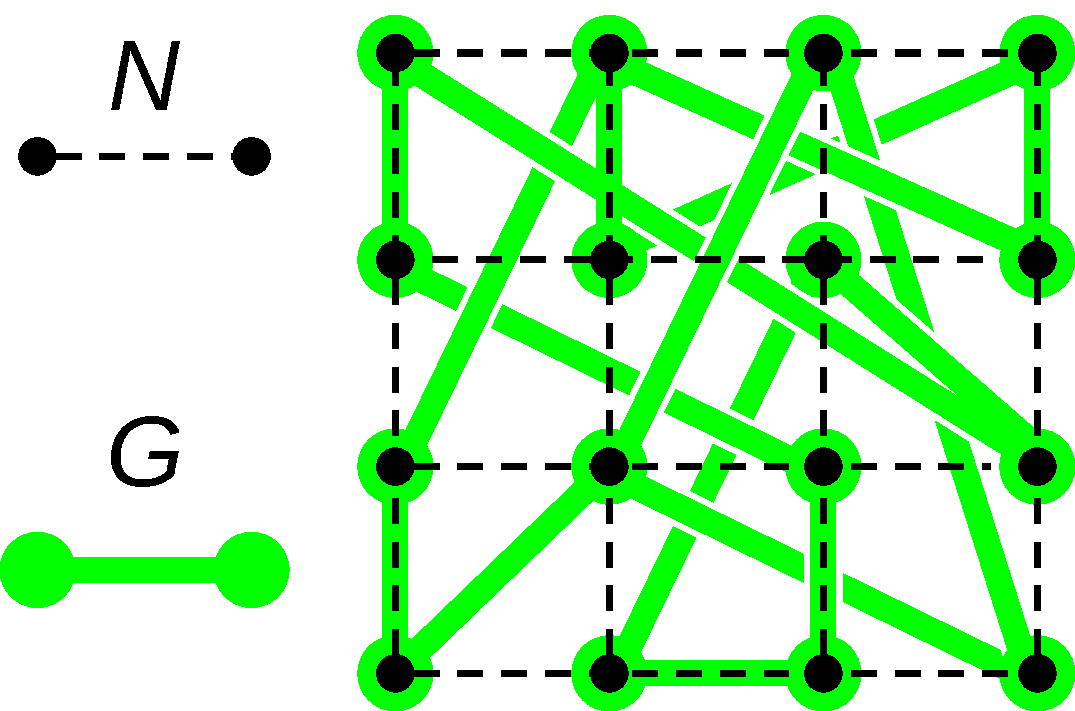
\includegraphics[width=\linewidth]{nandg}
\caption{
TODO
}
\label{fig:nandg}
\end{center}
\end{figure}


Edges in the graph $G$ do not represent a physical interconnect.
Instead, edges $\{\hat{a}, \hat{b}\} \in E(G)$ represent a close-coordination relationship where node $\hat{a}$ frequently interacts with (i.e., dispatches messages to) the destination node $\hat{b}$.
Figure \ref{fig:nandg} illustrates the relationship between $N$ and $G$.

Let $\hat{d}(\hat{a},\hat{b})$ denote distance between vertices $\hat{a}$ and $\hat{b}$ with respect to the graph $G$.
That is, the number of graph edges traversed on a shortest-path route between $\hat{a}$ and $\hat{b}$ over $G$.
In a small-world network, typical graph distance scales proportionally with the logarithm of network size \citeinappendix{watts1998collective}.
In our case, for arbitrary $\hat{a},\hat{b} \in V(G)$,
\begin{align} \label{eqn:smallworld_prop}
\bar{\hat{d}}(\hat{a},\hat{b}) \propto \log(|V(G)|).
\end{align}

Suppose we have a small-world graph $G$ constructed over a mesh $N$ (as in Figure \ref{fig:nandg}) using the Watts–Strogatz algorithm.
In this procedure, vertices in $V(G)$ corresponding to neighboring computational nodes in $V(N)$ are wired together to form a lattice with mean degree $k$.
Then, for every vertex $v \in V(G)$, each edge $\{x, y\} \in E(G)$ containing $v$ is reconfigured with probability $0 < \beta < 1$ to connect $v$ to a randomly-chosen node $w \in V(G)$.

Before reconfiguration, the total wiring cost of $G$ with respect to hops over $N$ was proportional to $|V(G)|$.

Recall that, with mesh dimensionality $r$ we know that for a pair of arbitrary nodes $a,b \in V(N)$,
\begin{align*}
\bar{d}(a, b) \propto |V(N)|^{\frac{1}{r}} \times r.
\end{align*}

So, after rewiring, the total wiring cost $w$ of $G$ with respect to hops over $N$ can be calculated as
\begin{align*}
  \beta |V(G)| \times |V(N)|^{\frac{1}{r}} \times r + (1 - \beta) |V(G)|.
  %\\
  % \beta |V(N)| \times |V(N)|^{\frac{1}{r}} \times r + (1 - \beta) |V(N)|.
  % \beta |V(N)|^{\frac{r+1}{r}} \times r + (1 - \beta) |V(N)|.
\end{align*}

So, $w \in \Omega \Big( |V(N)|^{\frac{r+1}{r}} \times r \Big).$

In this graph, the number of edges is proportional to the graph size $n$.

With bounded mean degree, we have $|E(G)| \propto |V(G)|$ so we can establish the following lower bound on mean wiring cost per edge of $G$ with respect to hops over $N$,
\begin{align*}
\Omega \Big( |V(G)|^{\frac{1}{r}}| \times r \Big).
\end{align*}

Note that, with the introduction of log-time hierarchical hardware interconnects into $N$ the mean wiring cost per edge of $G$ with respect to hops over $N$ is bounded in the worst case by $\Omega \Big( \log |V(G)| \Big)$.


% \begin{figure}[!htbp]
\begin{center}
\begin{subfigure}[b]{0.49\columnwidth}
  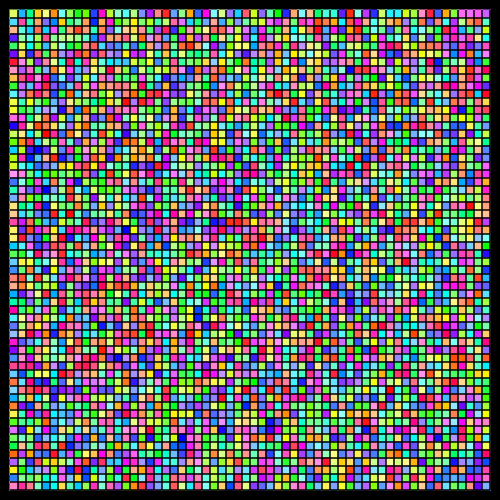
\includegraphics[width=\columnwidth]{source_hash=de48c04-dirty_emp_hash=1c7cb544-clean_title=channel_viz+treat=resource-wave__channelsense-yes__nlev-two+seed=1+update=0}
  \caption{Update 0; gen. 0}
  \label{fig:TODO}
\end{subfigure}
\begin{subfigure}[b]{0.49\columnwidth}
  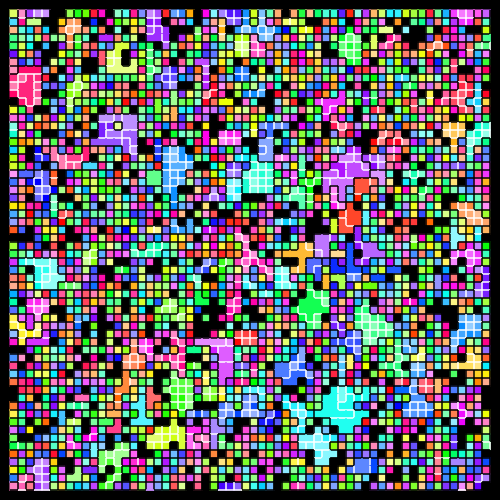
\includegraphics[width=\columnwidth]{source_hash=de48c04-dirty_emp_hash=1c7cb544-clean_title=channel_viz+treat=resource-wave__channelsense-yes__nlev-two+seed=1+update=2500}
  \caption{Update 2.5k; gen. TODO}
  \label{fig:TODO}
\end{subfigure}
\begin{subfigure}[b]{0.49\columnwidth}
  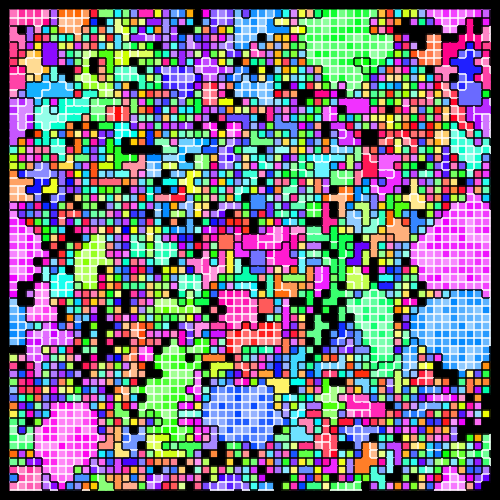
\includegraphics[width=\columnwidth]{source_hash=de48c04-dirty_emp_hash=1c7cb544-clean_title=channel_viz+treat=resource-wave__channelsense-yes__nlev-two+seed=1+update=5000}
  \caption{Update 5k; gen. TODO}
  \label{fig:TODO}
\end{subfigure}
\begin{subfigure}[b]{0.49\columnwidth}
  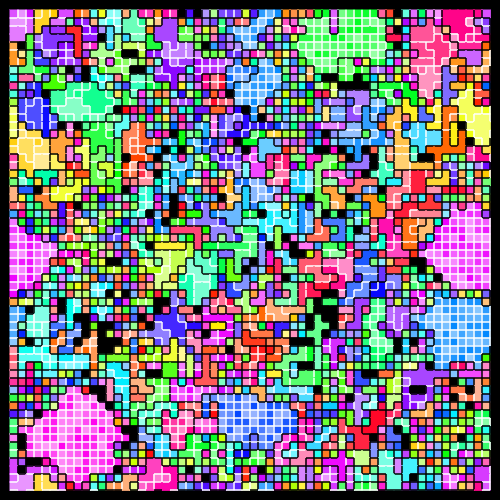
\includegraphics[width=\columnwidth]{source_hash=de48c04-dirty_emp_hash=1c7cb544-clean_title=channel_viz+treat=resource-wave__channelsense-yes__nlev-two+seed=1+update=7500}
  \caption{Update 7.5k; gen. TODO}
  \label{fig:TODO}
\end{subfigure}
\begin{subfigure}[b]{0.49\columnwidth}
  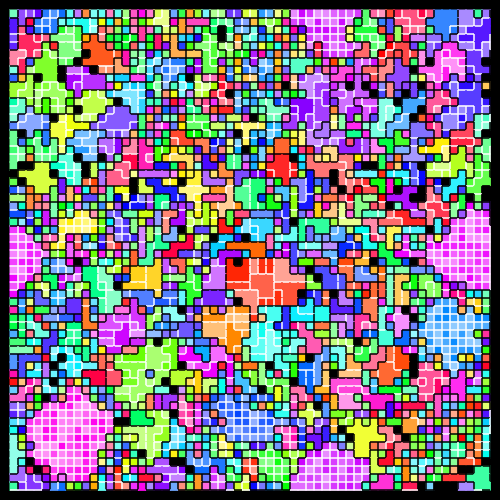
\includegraphics[width=\columnwidth]{source_hash=de48c04-dirty_emp_hash=1c7cb544-clean_title=channel_viz+treat=resource-wave__channelsense-yes__nlev-two+seed=1+update=10000}
  \caption{Update 10k; gen. TODO}
  \label{fig:TODO}
\end{subfigure}
\begin{subfigure}[b]{0.49\columnwidth}
  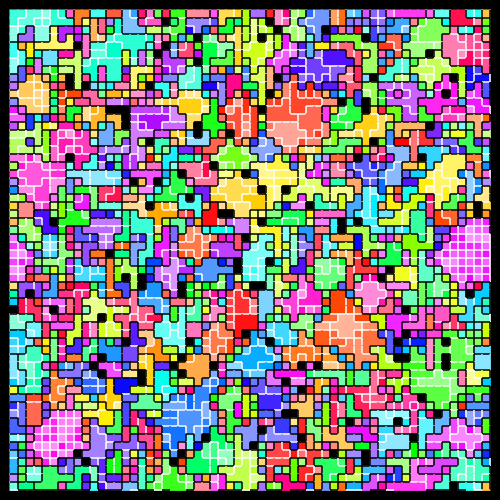
\includegraphics[width=\columnwidth]{source_hash=de48c04-dirty_emp_hash=1c7cb544-clean_title=channel_viz+treat=resource-wave__channelsense-yes__nlev-two+seed=1+update=20000}
  \caption{Update 20k; gen. TODO}
  \label{fig:TODO}
\end{subfigure}
\begin{subfigure}[b]{0.49\columnwidth}
  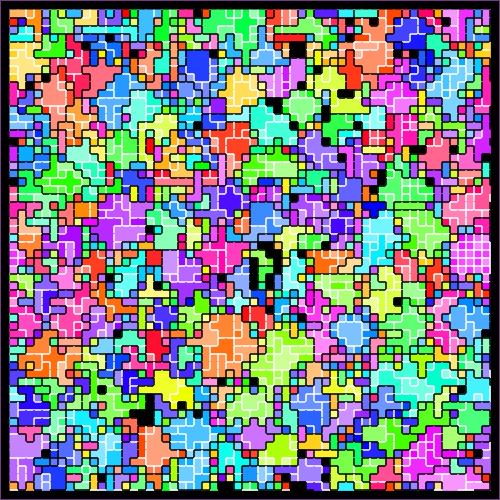
\includegraphics[width=\columnwidth]{source_hash=de48c04-dirty_emp_hash=1c7cb544-clean_title=channel_viz+treat=resource-wave__channelsense-yes__nlev-two+seed=1+update=30000}
  \caption{Update 30k; gen. TODO}
  \label{fig:TODO}
\end{subfigure}
\begin{subfigure}[b]{0.49\columnwidth}
  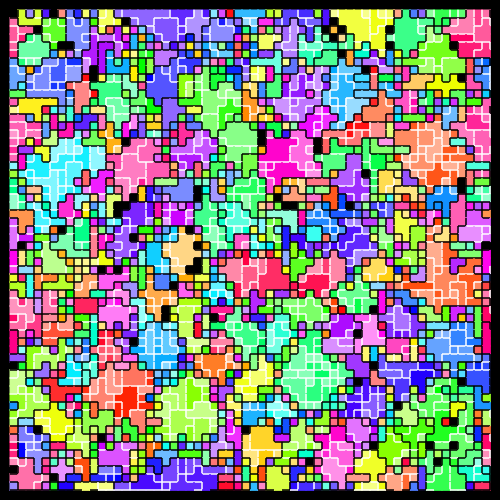
\includegraphics[width=\columnwidth]{source_hash=de48c04-dirty_emp_hash=1c7cb544-clean_title=channel_viz+treat=resource-wave__channelsense-yes__nlev-two+seed=1+update=50000}
  \caption{Update 50k; gen. TODO}
  \label{fig:TODO}
\end{subfigure}
\caption{
Progression of of same-channel level-zero and level-one signaling networks states in an evolutionary run.
In the "Channel Viewer", low-level groups are coded by color saturation (divided by white lines) and high-level groups are coded by color hue (divided by black lines).
Black grid tiles represent empty channel ID.
}
\label{fig:grid_progression}
\end{center}
\end{figure}


\subsection{Case Study: Interconnect Resource Sharing}

\begin{figure}[!htbp]
\begin{center}
\begin{subfigure}[b]{\linewidth}
  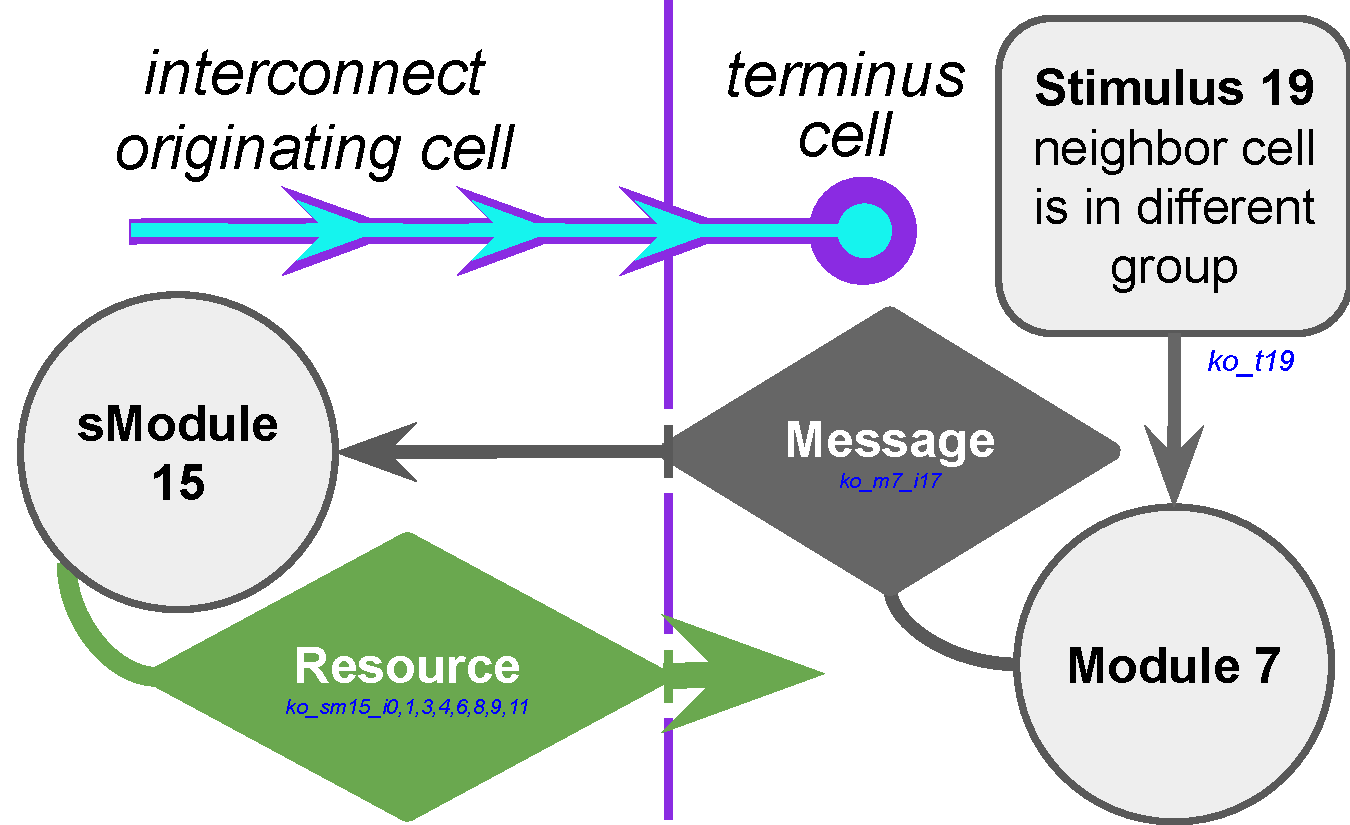
\includegraphics[width=\linewidth,clip]{batch=1042+step=1024+pop=3/1042_diagram}
  \caption{TODO}
  \label{fig:TODO}
\end{subfigure}
\begin{subfigure}[b]{0.33\linewidth}

  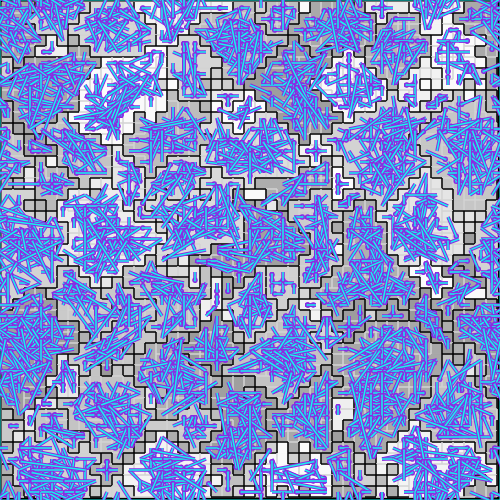
\includegraphics[width=\linewidth,trim={0 100 100 0},clip]{batch=1042+step=1024+pop=3/seed=1+title=established-interconnect+treat=batch_1042,step_1024,pop_3,id1_wt+update=4990+_emp_hash=0c549f0-clean+_source_hash=a6072a6-clean+ext=}
  \caption{TODO}
  \label{fig:TODO}
\end{subfigure}
\begin{subfigure}[b]{0.33\linewidth}
  
\includegraphics[width=\linewidth,trim={0 100 100 0},clip]{batch=1042+step=1024+pop=3/seed=1+title=channel+treat=batch_1042,step_1024,pop_3,id1_wt+update=4990+_emp_hash=0c549f0-clean+_source_hash=a6072a6-clean+ext=}
  \caption{TODO}
  \label{fig:TODO}
\end{subfigure}
\begin{subfigure}[b]{0.33\linewidth}
  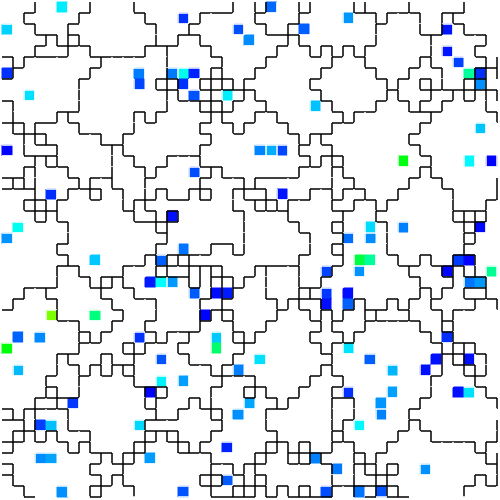
\includegraphics[width=\linewidth,trim={0 100 100 0},clip]{batch=1042+step=1024+pop=3/seed=1+title=interconnect-shared-resource+treat=batch_1042,step_1024,pop_3,id1_wt+update=4990+_emp_hash=0c549f0-clean+_source_hash=a6072a6-clean+ext=}
  \caption{TODO}
  \label{fig:TODO}
\end{subfigure}
\begin{subfigure}[b]{0.33\linewidth}
  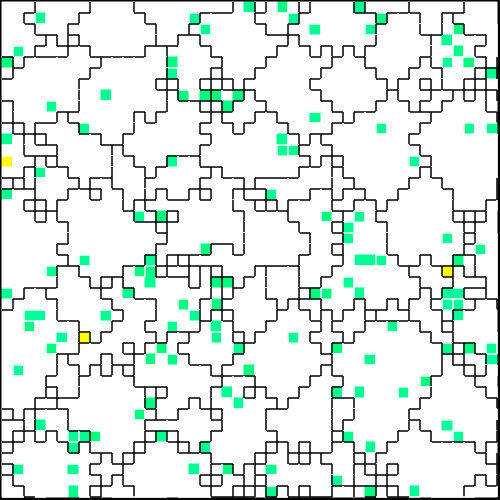
\includegraphics[width=\linewidth,trim={0 100 100 0},clip]{batch=1042+step=1024+pop=3/seed=1+title=interconnect-sharing-fraction+treat=batch_1042,step_1024,pop_3,id1_wt+update=4990+_emp_hash=0c549f0-clean+_source_hash=a6072a6-clean+ext=}
  \caption{TODO}
  \label{fig:TODO}
\end{subfigure}
\caption{
TODO
}
\label{fig:case_study_1042}
\end{center}
\end{figure}


This case study was drawn from epoch 24 of batch 42 of the initial set of evolutionary runs.
We initially considered it for further study due to the presence of widespread over-interconnect resource sharing.
After preliminary knockout experiments confirmed the adaptive significance of both over-interconnect resource-sharing and over-interconnect messaging, we set aside the strain for a case study.
The evolutionary history preceding this case study consumed approximately 96 hours of wall-clock time and 736 compute-core hours.
Approximately TODO simulation updates and TODO cellular generations elapsed.
You can view the strain this case study characterizes in a live in-browser simulation at \url{https://mmore500.com/hopto/8}

Our first step was to evaluate whether intercellular nature of over-interconnect messaging and resource sharing contributed to the strain's fitness.
(It is possible that messaging and/or resource sharing behaviors might generate stimuli on the recipient or side-effects on the sender that have adaptive consequences whether or not the sender and recipient are distinct cells;
in such a scenario, cells would be just as well off sending messages and/or resource to themselves.)
We performed several competition experiments between between the wild-type strain and variants where interconnect messaging and resource sharing was altered to be intracellular instead of intercellular.
At the end of competition experiments, we evaluated the relative abundances of wild-type and variant strains.
In the first variant strain we tested, all outgoing over-interconnect messages were delivered to the sending cell.
In 16 out of 16 one-hour competition runs that were seeded half-and-half with the wild-type and variant strains, the wild-type strain drove the variant strain to extinction (one-tailed binomial test; $p < 0.0001$; 290 S.D 17 cell gens elapsed).
We observed a similar outcome with a second variant strain where all outgoing over-interconnect resource sharing was rerouted back to the sending cell (14/16 variant strain extinctions; 16/16 wild-type prevalence; 289 S.D. 25 cell gens elapsed).
Finally, a third variant strain where both over-interconnect messaging and over-interconnect resource sharing were returned to the sending cell exhibited the same outcome (16/16 variant strain extinctions; 300 S.D. 23 cell gens elapsed).
The intercellular natures of both over-interconnect messaging and resource sharing appear essential to fitness.

Next, we took a closer look at the evolved cellular mechanisms controlling over-interconnect messaging and resource sharing.
We monitored hardware execution of the wild-type strain in a monoculture population to detect which signals, messages, and fork/call instructions activated each SignalGP module.
We manually cross-referenced this information with a human-readable printout of the strain's genetic program to construct hypothesized mechanism shown in Figure \ref{fig:case_study_1042}.
We hypothesize that cells at the periphery of a registered kin groups send messages backwards over incoming interconnects that induce interconnect-originating cells to send them resource.
Such a mechanism could preferentially increase resource availability at the group periphery, a region where cell-cell conflict is likely elevated.

We performed a series of four-hour competition experiments between wild type and knockout strains to confirm the adaptive nature of each component of this mechanism.
We began by re-routing stimulus 19, which alerts cells to a non-registered-kin neighbor, to activate a known no-op module.
This knockout strain experienced decreased fitness compared to the wild-type strain (16/16 knockout strain extinctions; one-tailed binomial test; $p < 0.0001$; 1996 S.D. 280 cell gens elapsed; \url{https://mmore500.com/hopto/ak}).
Next, we replaced the over-interconnect messaging instruction that triggers over-interconnect resource-sharing with a no-op instruction.
This knockout strain also experienced decreased fitness (16/16 knockout strain extinctions; 1932 S.D. 223 cell gens elapsed; \url{https://mmore500.com/hopto/al}).
We then replaced all eight copies of the over-interconnect resource-sharing instruction triggered by the over-interconnect messaging with no-op instructions, once more yielding a strain with diminished fitness (16/16 knockout strain extinctions; 1860 S.D. 370 cell gens elapsed; \url{https://mmore500.com/hopto/am}).
Finally, we confirmed the soundness of our fitness competition methodology by running control wild-type versus wild-type competitions.
As expected, we observed no effect of strain ID on competition dominance (8/16 knockout strain extinctions; 8/16 wild-type strain extinctions; one-tailed binomial test; $p = 0.60$; 1738 S.D. 217 cell gens elapsed; \url{https://mmore500.com/hopto/aj})

\subsection{Case Study: Interconnect Messaging}

\begin{figure}[!htbp]

\begin{center}
\begin{subfigure}[b]{\linewidth}
  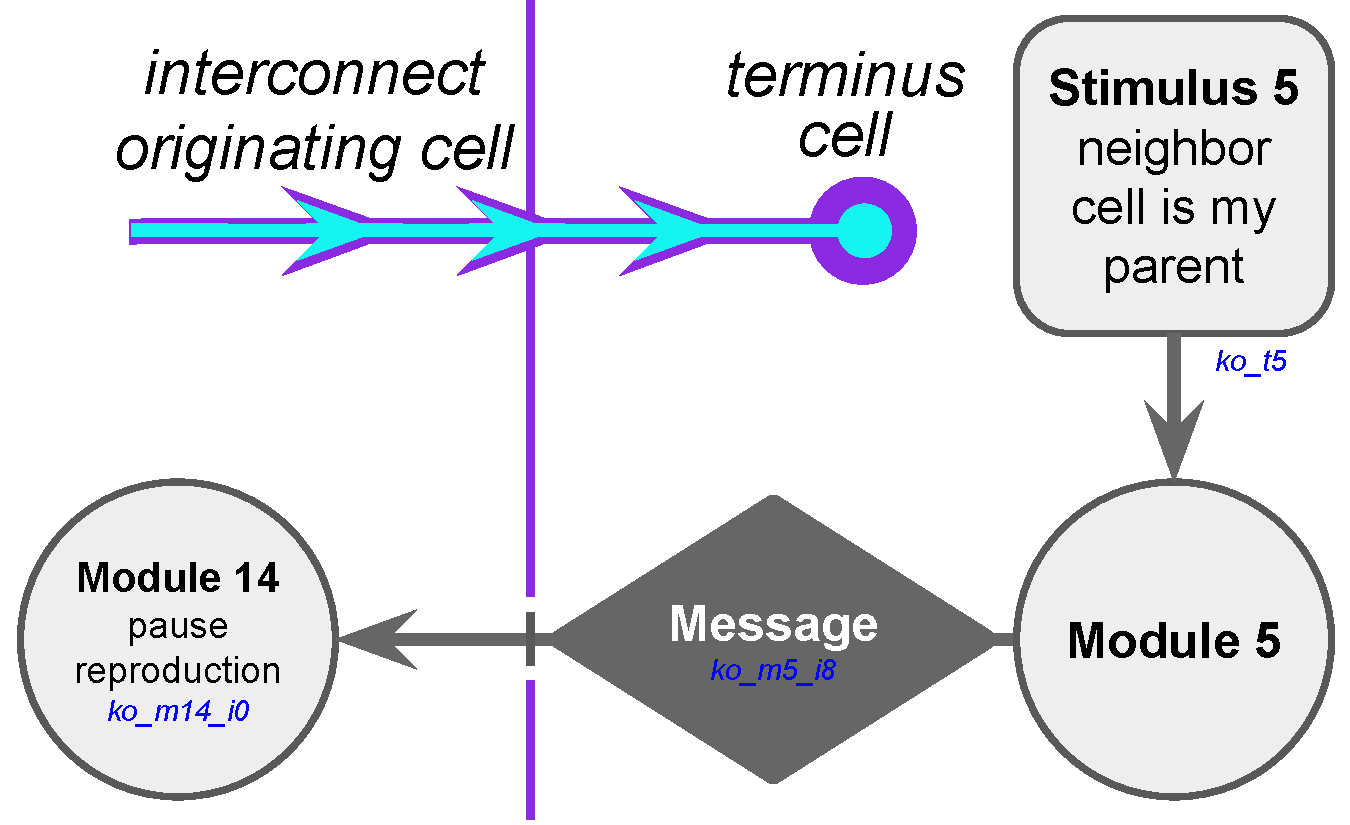
\includegraphics[width=\linewidth,clip]{batch=2032+step=1018+pop=0/2032_diagram}
  \caption{Hypothesized selective reproduction pausing mechanism}
  \label{fig:mechanism2}
\end{subfigure}
\begin{subfigure}[b]{0.45\linewidth}
  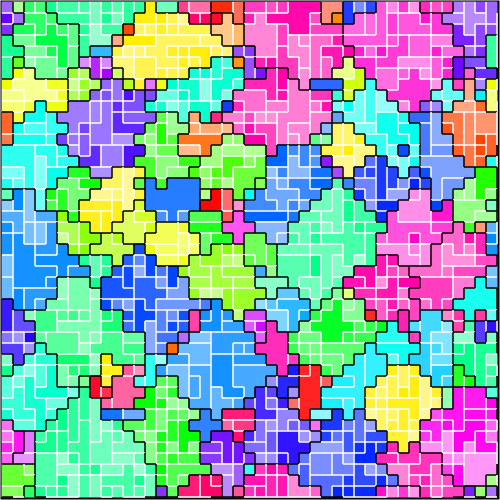
\includegraphics[width=\linewidth,trim={0 200 200 0},clip]{batch=2032+step=1018+pop=0/seed=1+title=channel+treat=batch_2032,step_1018,pop_1,id1_wt+update=5000+_emp_hash=0c549f0-clean+_source_hash=d50b431-dirty+ext=}
  \caption{Kin groups}
  \label{fig:kingroups2}
\end{subfigure}
\begin{subfigure}[b]{0.45\linewidth}
  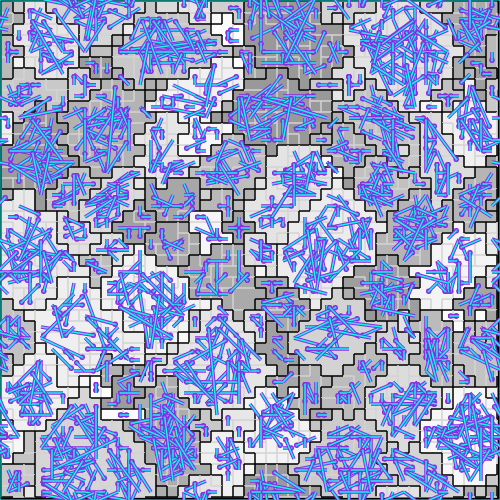
\includegraphics[width=\linewidth,trim={0 200 200 0},clip]{batch=2032+step=1018+pop=0/seed=1+title=established-interconnect+treat=batch_2032,step_1018,pop_1,id1_wt+update=5000+_emp_hash=0c549f0-clean+_source_hash=d50b431-dirty+ext=}
  \caption{Established interconnects}
  \label{fig:establishedinterconnects2}
\end{subfigure}
\begin{subfigure}[b]{0.45\linewidth}
  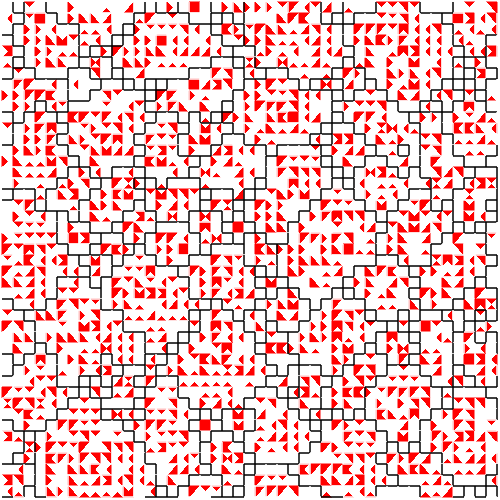
\includegraphics[width=\linewidth,trim={0 200 200 0},clip]{batch=2032+step=1018+pop=0/seed=1+title=parent-cell-of+treat=batch_2032,step_1018,pop_1,id1_wt+update=5000+_emp_hash=0c549f0-clean+_source_hash=d50b431-dirty+ext=}
  \caption{Spatial distriubiton of stimulus 5TODO fix}
  \label{fig:t5distribution}
\end{subfigure}
\begin{subfigure}[b]{0.45\linewidth}
  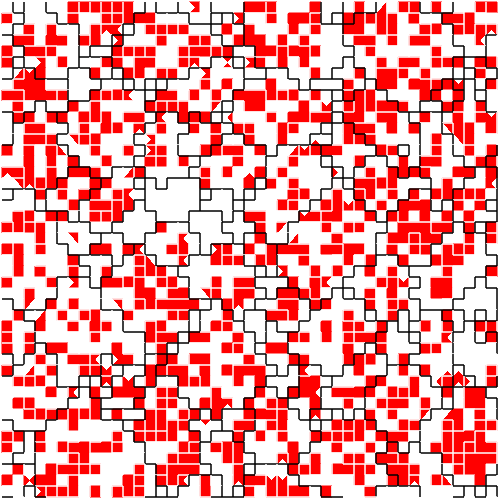
\includegraphics[width=\linewidth,trim={0 200 200 0},clip]{batch=2032+step=1018+pop=0/seed=1+title=reproductive-pause-level-0+treat=batch_2032,step_1018,pop_1,id1_wt+update=5000+_emp_hash=0c549f0-clean+_source_hash=d50b431-dirty+ext=}
  \caption{Spatial distribution of module 14 execution}
  \label{fig:m14distribution}
\end{subfigure}
\caption{
Batch 2032 case study overview.
Figures \ref{fig:kingroups2} through \ref{fig:m14distribution} are generated from a snapshot of a wild-type strain monoculture population.
In these images, each grid tile represents an individual cell.
Cells are organized into kin groups, color-coded by hue in Figure \ref{fig:kingroups2}.
Established interconnects are overlaid in blue on Figure \ref{fig:establishedinterconnects2}.
In Figures \ref{fig:t5distribution} and \ref{fig:m14distribution}, kin groups are outlined in black.
Figure \ref{fig:t5distribution} highlights cells that are sending resource over-interconnect.
Figure \ref{fig:m14distribution} highlights cells that are receiving resource over-interconnect.
You can view an animation of the wild-type monoculutre at \url{https://mmore500.com/hopto/an}.
}
\label{fig:case_study_2032}
\end{center}
\end{figure}


overview animation \url{https://mmore500.com/hopto/an}

This case study was drawn from time point 18 of a batch of the secondary set of runs.
72 compute hours, TODO cellular generations elapsed.
You can view this strain in a live in-browser simulation at \url{https://mmore500.com/hopto/7}.

knockout experiments
\begin{itemize}
  \item wt vs wt (5/16 successes; \url{https://mmore500.com/hopto/9}; 12/16 coalesced; 408 S.D. 43 cell gen)
  \item m5/i8 knockout (16/16 success; \url{https://mmore500.com/hopto/aa}; 16/16 coalesced; 416 S.D. 58 cell gen)
  \item m14/i0 (16/16 success; \url{https://mmore500.com/hopto/ab}; 16/16 coalesced; 401 S.D. 29 cell gen)
  \item self-messaging (16/16 and 16/16; 5/16 coalesced and 2/16 coalesced; 54 S.D. 2 cell gen and 52 S.D. 3 cell gen)
  \item m5/i8 replace with
  \begin{itemize}
	\item call (16/16; \url{https://mmore500.com/hopto/ac}; 16/16 coalesced; 378 S.D. 42 cell gen)
    \item fork (16/16; \url{https://mmore500.com/hopto/ad} 16/16 coalesced; 377 S.D. 37 cell gen)
    \item sendinternal (16/16; \url{https://mmore500.com/hopto/ae}; 16/16 coalesced; 406 S.D 39 cell gen)
    \item bcstinternal (16/16; \url{https://mmore500.com/hopto/af}; 16/16 coalesced; 422 S.D 30 cell gen)
    \item sendexternal (16/16; \url{https://mmore500.com/hopto/ag}; 16/16 coalesced; 377 S.D. 37 cell gen)
    \item bcstexternal (16/16; \url{https://mmore500.com/hopto/ah}; 16/16 coalesced; 440 S.D. 32 cell gen)
    \item bcstfwdspiker (10/16; \url{https://mmore500.com/hopto/ai}; 14/16 coalesced; 410 S.D. 50 cell gen)
  \end{itemize}
  \item t5 always (16/16; 16/16 coalesced; 48 S.D. 3 cell gen)
  \item t5 invert (16/16; 16/16 coalesced; 48 S.D 3 cell gen)
  \item t5 never (16/16; 16/16 coalesced; 52 S.D. 3 cell gen)
  \item trigger 5 stochastic (observe trigger frequency of 22729/(22729+82571) between 1000 and 1100 updates in a monoculture population) (16/16; 16/16 coalesced; 62 S.D. 3 cell gen)
  \item remapping trigger 5 to activate module stochastic triggering of module 14 only on pointer between 1000 (238940 hits) and 1100 (267392 hits) updates -> 28452 / (12*45*45*4) = 0.292716 (16/16; 16/16 coalesced; 58 S.D. 2 cell gen)
\end{itemize}

%TODO Figure \ref{fig:case_study_1042}

